% !TeX root = ../note.tex
\subsection{Обзор существующих аналогов}\label{sec:analysis:analogues}

В данном разделе рассмотрим существующие аналоги, а именно системы, обладающие механизмами для создания ордеров, совершения сделок и другим соответствующим функционалом.

% \subsubsection{} Jira\label{sec:analysis:analogue_1}
\bigskip
\textbf{Jira}

Jira~\cite{analogue_1} позиционируется как коммерческая система отслеживания ошибок, разработана компанией Atlassian. Основной элемент учёта в системе — задача, которая содержит название проекта, тему, тип, приоритет, компоненты и содержание. Она может быть расширена дополнительными полями, различными приложениями (например — фотографиями, скриншотами и т.д.) или комментариями. Среди возможностей данной программы:
\begin{itemize}
    \item Kanban-доска — помогают команде обеспечить прозрачность работы над проектом, оптимизировать рабочий процесс, распределить задачи из списка нерешённых задач. Пример такой доски представлен на рисунке~\ref{fig:analysis:analogue_1:picture};
    \item Scrum-доска — позволяет управлять сложным проектом, объединить команды из разных направлений разработки продукта для достижений одной цели;
    \item отчёты формируются при помощи виджетов на панели дашбордов и могут содержать информацию о проекте в целом или об отдельных его элементах. Отчёты визуализируются в графики и диаграммы.
\end{itemize}

\begin{figure}[ht]
    \centering
	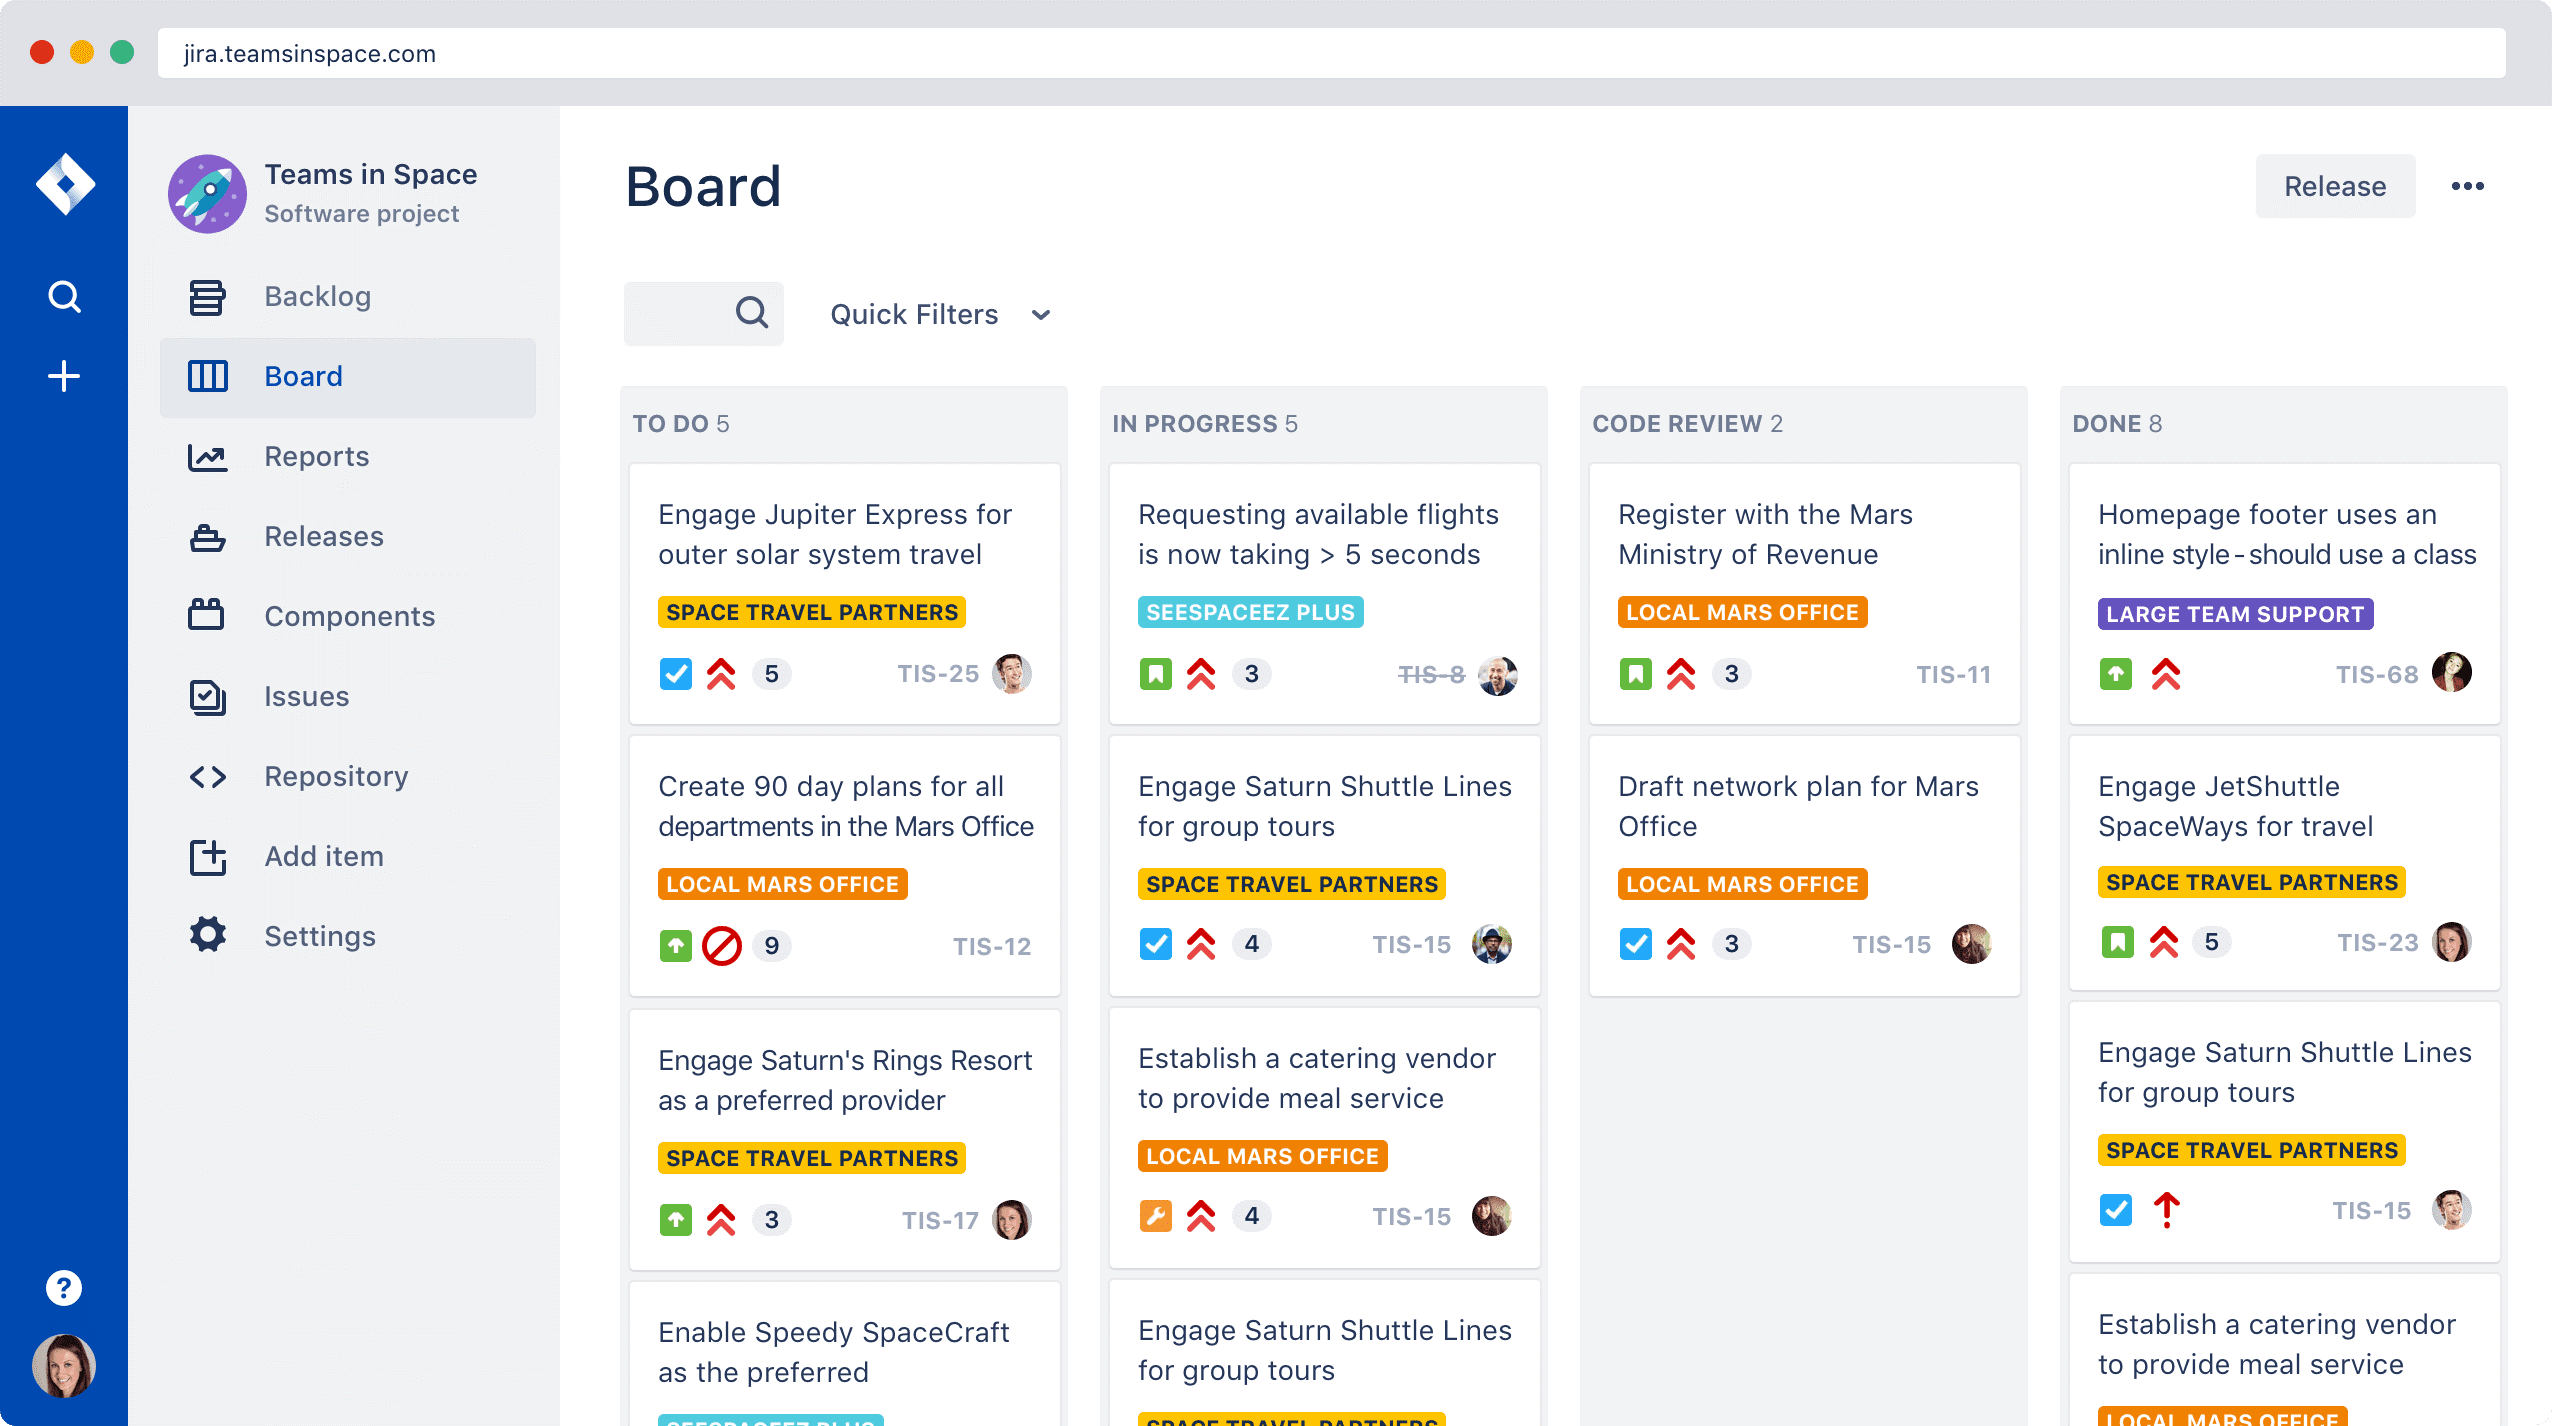
\includegraphics[width=\textwidth]{analogue_1.png}
	\caption{Пример Kanban-доски в системе Jira}\label{fig:analysis:analogue_1:picture}
\end{figure}

Из плюсов данного проекта можно отметить:
\begin{itemize}
    \item огромное количество функционала для эффективной работы над проектами;
    \item поддержка интеграций с множеством инструментов для разработки и других сервисов;
    \item широкая кастомизация, которая позволяет с лёгкостью адаптироваться под нужды конкретных заказчиков.
\end{itemize}

К минусам данного ПО можно отнести:
\begin{itemize}
    \item высокая цена с привязкой к количеству пользователей;
    \item сложный интерфейс;
    \item отсутствие по умолчанию функционала для работы с персоналом.
\end{itemize}

\bigskip
\textbf{YouTrack}

YouTrack — коммерческая система отслеживания ошибок, разработана компанией JetBrains~\cite{analogue_2}. Система поддерживает поисковые запросы, автодополнение, создание пользовательских рабочих процессов. Стандартные интеграции YouTrack включают импорт из Jira, интеграции с электронными почтовыми ящиками, c Zendesk, единую рабочую среду с Upsource и TeamCity, а также встроенную интеграцию с системами контроля версий GitHub, BitBucket и GitLab.

\begin{figure}[ht]
    \centering
	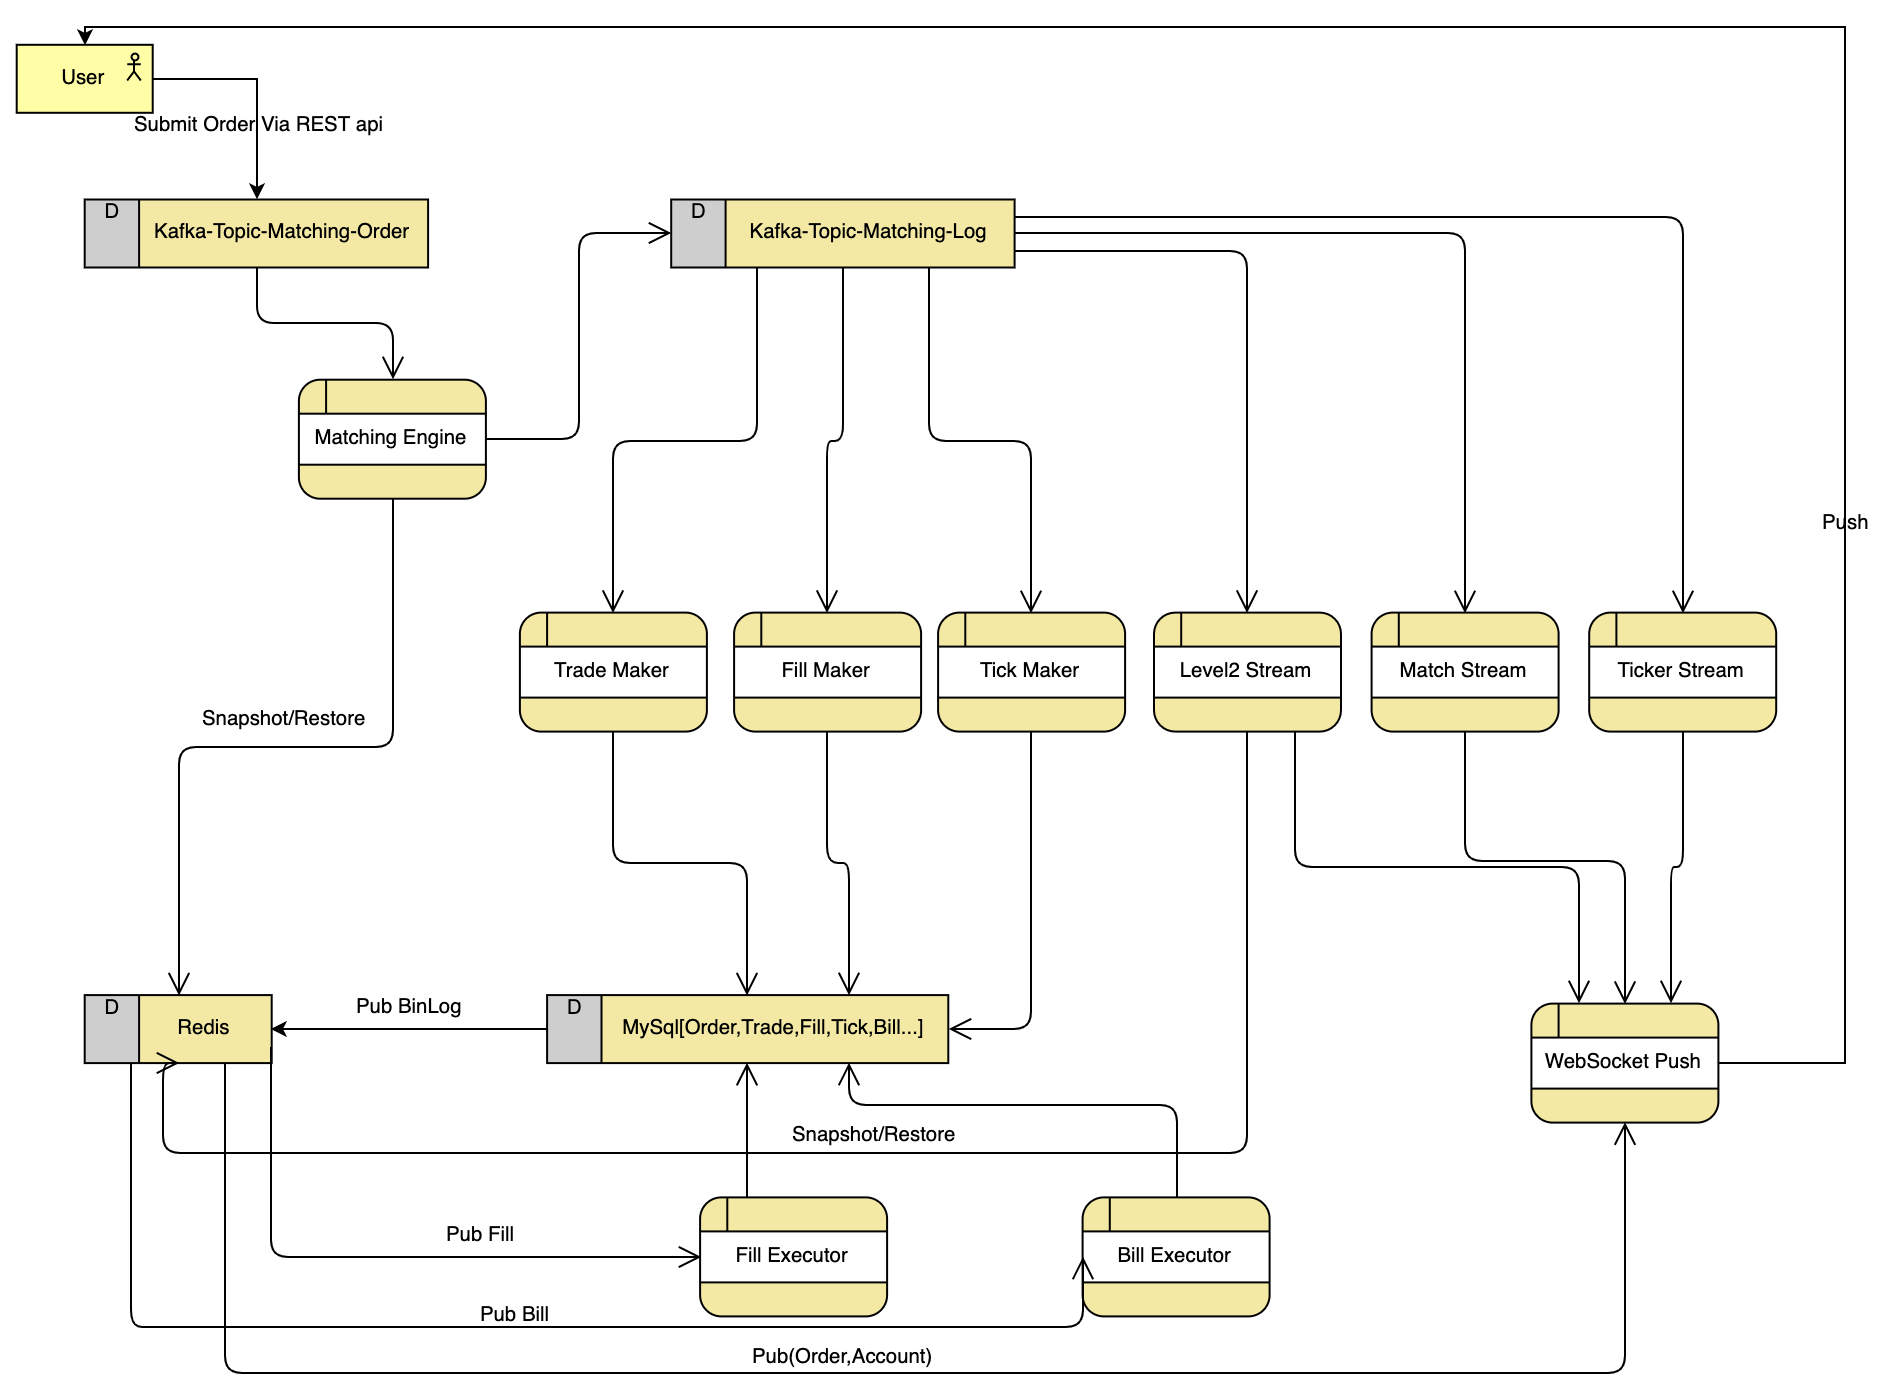
\includegraphics[width=\textwidth]{analogue_2.png}
	\caption{Пример доски в системе YouTrack}\label{fig:analysis:analogue_2:picture}
\end{figure}

В данном проекте можно отметить как плюсы следующее:
\begin{itemize}
    \item Scrum и Kanban доски для визуализации процесса разработки. Пример доски представлен на рисунке~\ref{fig:analysis:analogue_2:picture};
    \item интеллектуальный поиск при помощи поисковых запросов с подсказками и подсветкой ошибок;
    \item возможность применения команд для быстрого изменения нескольких задач сразу;
    \item Экспорт в CSV;
    \item поддержка интеграции с IDE от JetBrains: IntelliJ IDEA, PhpStorm, WebStorm, PyCharm, RubyMine, CLion, Rider, GoLand и AppCode.
\end{itemize}

К минусам данного ПО можно отнести:
\begin{itemize}
    \item высокая цена;
    \item небольшие проблемы с производительностью;
    \item отсутствие функционала для работы с персоналом.
\end{itemize}

\bigskip
\textbf{Trello}

Trello — облачная программа для управления проектами небольших групп, разработанная Fog Creek Software~\cite{analogue_3}. В Trello основной упор сделан на пачки карточек. Каждая пачка показывает состояние любого проекта. Карточки имеют множество возможностей. Они предназначены для обсуждений, голосований, загрузки файлов и данных. Есть возможность задавать дедлайны, назначать текстовые и цветовые метки.

\begin{figure}[ht]
    \centering
	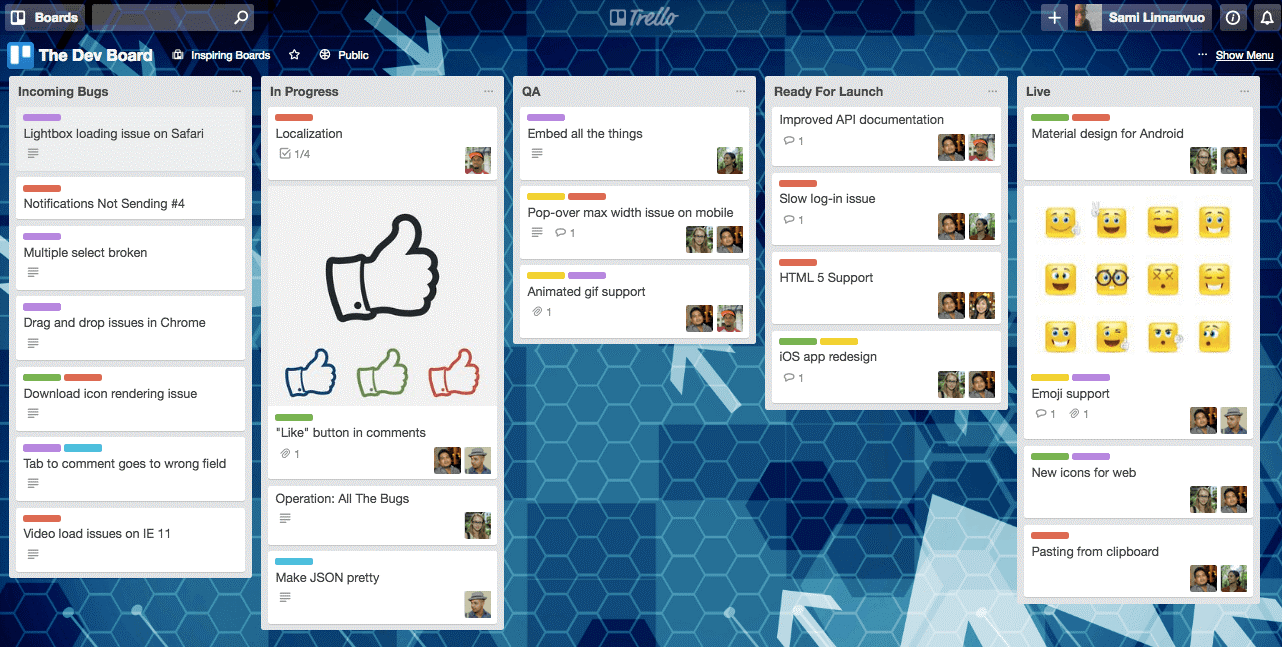
\includegraphics[width=\textwidth]{analogue_3.png}
	\caption{Пример доски в системе Trello}\label{fig:analysis:analogue_3:picture}
\end{figure}

Из сильных сторон проекта можно выделить:
\begin{itemize}
    \item Kanban-доски, которые помогают команде обеспечить прозрачность работы над проектом, оптимизировать рабочий процесс, распределить задачи из списка нерешённых задач. Пример такой доски представлен на рисунке~\ref{fig:analysis:analogue_3:picture};
    \item удобная и широко настраиваемая система уведомлений;
    \item наличие мобильной версии;
    \item низкая цена.
\end{itemize}

К минусам данного ПО можно отнести:
\begin{itemize}
    \item малое количество штатных средств для форматирования текста на карточках;
    \item малая интеграция со сторонними сервисами;
    \item отсутствие функционала для работы с персоналом.
\end{itemize}

\bigskip
\textbf{Azure DevOps Server}

Azure DevOps Server – продукт корпорации Microsoft, представляющий собой комплексное решение~\cite{analogue_4}, объединяющее в себе систему управления версиями, сбор данных, построение отчётов, отслеживание статусов и изменений по проекту и предназначенное для совместной работы над проектами по разработке программного обеспечения.

Из сильных сторон проекта можно отметить:
\begin{itemize}
    \item Kanban-доски, которые помогают команде обеспечить прозрачность работы над проектом, оптимизировать рабочий процесс, а также распределить задачи из списка нерешённых задач;
    \item Scrum-доска, которая позволяет управлять сложным проектом, объединить команды из разных направлений разработки продукта для достижений одной цели;
    \item возможность привязки программного кода к задачам при помощи собственного репозитория управления исходным кодом;
    \item автоматическое создание SharePoint-сайта для проекта, который может использоваться для отслеживания прогресса проекта, наблюдения за рабочими элементами и документами, представленными в библиотеке проекта.
\end{itemize}

К минусам данного ПО можно отнести:
\begin{itemize}
    \item очень высокая цена с привязкой к количеству пользователей;
    \item отсутствие функционала для работы с персоналом.
\end{itemize}
